\documentclass{article}
\usepackage{graphicx}
\setlength{\parindent}{0cm}

\usepackage{listings}
\usepackage{color}

\definecolor{dkgreen}{rgb}{0,0.6,0}
\definecolor{gray}{rgb}{0.5,0.5,0.5}
\definecolor{mauve}{rgb}{0.58,0,0.82}

\lstset{frame=tb,
  language=Matlab,
  aboveskip=3mm,
  belowskip=3mm,
  showstringspaces=false,
  columns=flexible,
  basicstyle={\small\ttfamily},
  numbers=none,
  numberstyle=\tiny\color{gray},
  keywordstyle=\color{blue},
  commentstyle=\color{dkgreen},
  stringstyle=\color{mauve},
  breaklines=true,
  breakatwhitespace=true
  tabsize=3
}

\begin{document}

\title{Matlab Fuzzy Clustering}
\author{Kyle Kastner and Hafez Bazrafshan}

\maketitle

\section*{K-means and Fuzzy C-means}
The K-means and fuzzy C-means algorithms \cite{ClusterAgg} are both unsupervised clustering
techniques. This means that any raw data can be fed to these algorithms, and
the resulting output will be "clustered" versions of the input. This is very
useful for detecting similarities between multiple sets of input data. One major difference is that
K-means has a lower algorithmic complexity than fuzzy clustering, making it easier to use on large datasets.
\vspace*{1\baselineskip}
Both K-means and fuzzy C-means require a number of
clusters parameter (K and C, respectively). This must be chosen \emph{apriori} 
(before) the algorithm is run.
The results from choosing a different number of clusters can vary wildly, and
techniques such as random search, the X-means algorithm, 
"Gaussian cluster splitting", the Bayesian information criteria (BIC), 
and Aikake information criteria are all used to choose the right number of
clusters for real world datasets. We plan to explore these automatic methods
during the Python portion of this homework.
\vspace*{1\baselineskip}

\section*{Datasets}
For this assignment, we have used synthetic datasets from 
University of Eastern Finland \cite{2DClust} (see Fig. ~\ref{fig:fez_2d_base})
, as well as accelerometer data from University of California - Irvine \cite{UCIML}
and kaggle.com. Using these datasets, we were able to find some results, but
there was a lot of difficulty in visualizing the high dimensional data, 
as well as achieving results consistent with visual inspection. 
We plan to expand our exploration of the topic in the python version of this homework.

\subsection*{2 Clusters}
Using K-means, we see that the 2 cluster datset has been decomposed into 2 groups (Fig. ~\ref{fig:fez_2d_kmeans}).
However, these groups do not align with what visual inspection shows to be the "right" clusters.
Fuzzy C-Means (Fig. ~\ref{fig:fez_2d_fuzzy}) performs slightly better, but still does not match visual expectations.
This is likely due to the non-circular nature of the bottom cluster - both K-means and fuzzy clustering make 
a circular assumption, whereas a technique such as Gaussian mixture modeling would likely be able to model
this curvature more effectively by changing the covariance structure of the clusters.

\begin{figure}[h!]
  \caption{A simple 2D dataset}
  \centering
    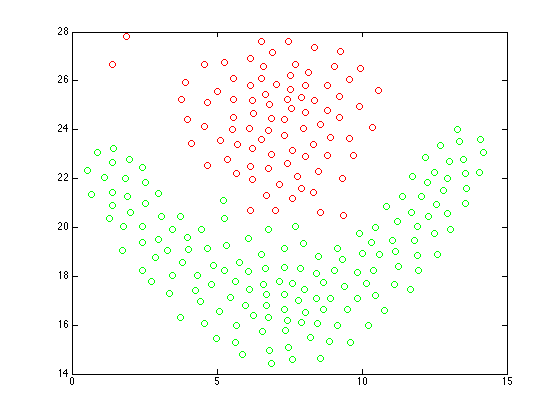
\includegraphics[width=0.85\textwidth]{fez_2d_base.png}
  \label{fig:fez_2d_base}
\end{figure}

\begin{figure}[h!]
  \caption{K-means clustering, 2D dataset}
  \centering
    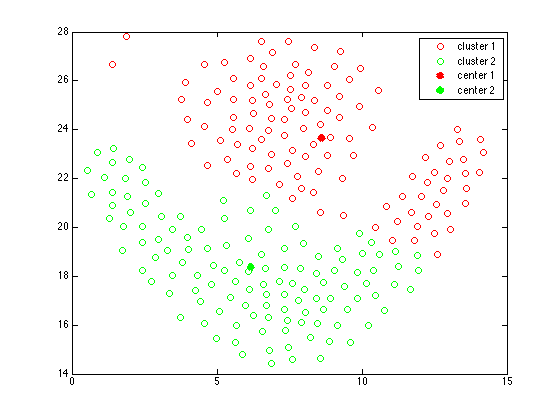
\includegraphics[width=0.85\textwidth]{fez_2d_kmeans.png}
  \label{fig:fez_2d_kmeans}
\end{figure}

\begin{figure}[h!]
  \caption{Fuzzy clustering, 2D dataset}
  \centering
    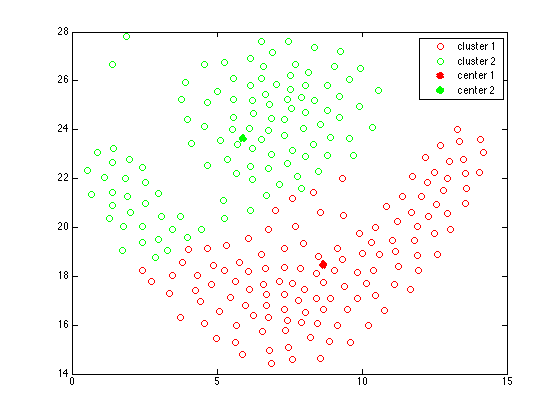
\includegraphics[width=0.85\textwidth]{fez_2d_fuzzy.png}
  \label{fig:fez_2d_fuzzy}
\end{figure}

\subsection*{7 Clusters}
Expanding our search to a more complex synthetic dataset (Fig. ~\ref{fig:fez_7clust_base}),
we once again performed K-means and fuzzy C-means clustering. Both K-means (Fig. ~\ref{fig:fez_7clust_kmeans}) 
and fuzzy C-means (Fig. ~\ref{fig:fez_7clust_fuzzy}) performed better on this dataset, however, the results
still do not match visual inspection. This could well be due to initialization issues with the clusters, as both 
K-means and fuzzy C-means algorithms are very sensitive to the starting position of the clusters. We attribute
the better performance here to the fact that the clusters are much more "circular" in nature.

\begin{figure}[h!]
  \caption{A 7 cluster dataset}
  \centering
    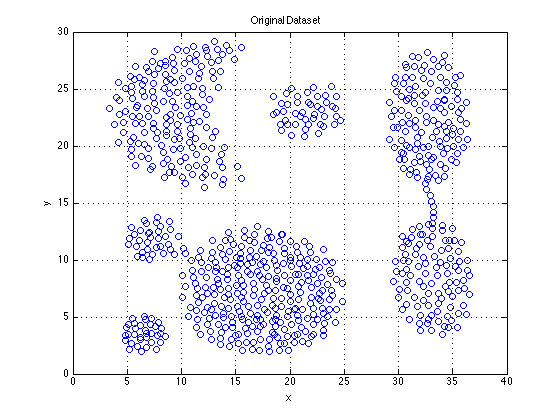
\includegraphics[width=0.85\textwidth]{fez_7clust_base.png}
  \label{fig:fez_7clust_base}
\end{figure}

\begin{figure}[h!]
  \caption{K-means clustering, 7 cluster dataset}
  \centering
    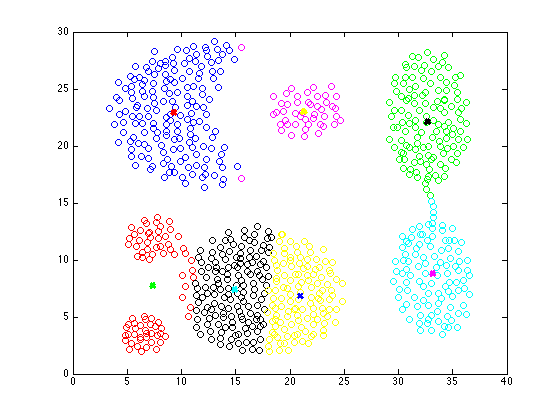
\includegraphics[width=0.85\textwidth]{fez_7clust_kmeans.png}
  \label{fig:fez_7clust_kmeans}
\end{figure}

\begin{figure}[h!]
  \caption{Fuzzy clustering, 7 cluster dataset}
  \centering
    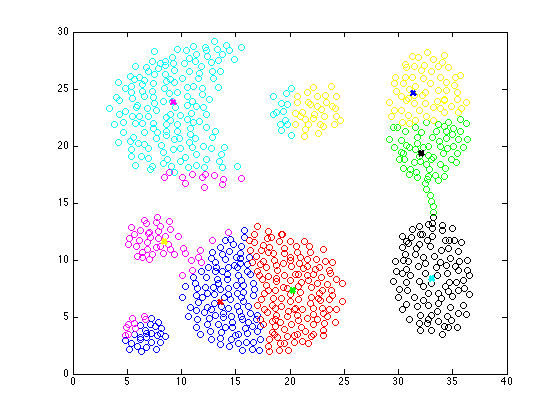
\includegraphics[width=0.85\textwidth]{fez_7clust_fuzzy.png}
  \label{fig:fez_7clust_fuzzy}
\end{figure}

\subsection*{Accelerometer}
Approaching the third dataset, \cite{Kaggle}, we must first project this matrix to 2 dimensions and plot it.
Using a technique called Principle Component Analysis, we can plot the data, the K-means clusters, and the 
fuzzy clusters in 2 dimensions (Fig. ~\ref{kyle_base}. This is a good start, but we plan to incorporate some other algorithms
during the second homework which should allow for more advanced analysis, with the eventual goal being Recognition
of individuals based on unique features of their accelerometer patterns (Fig. ~\ref{kyle_base}). The scatter plot legend is bugged
in octave < 3.8.0, but black is data, blue is kmeans, red is fuzzy.

\begin{figure}[h!]
  \caption{Accelerometer dataset, projected.}
  \centering
    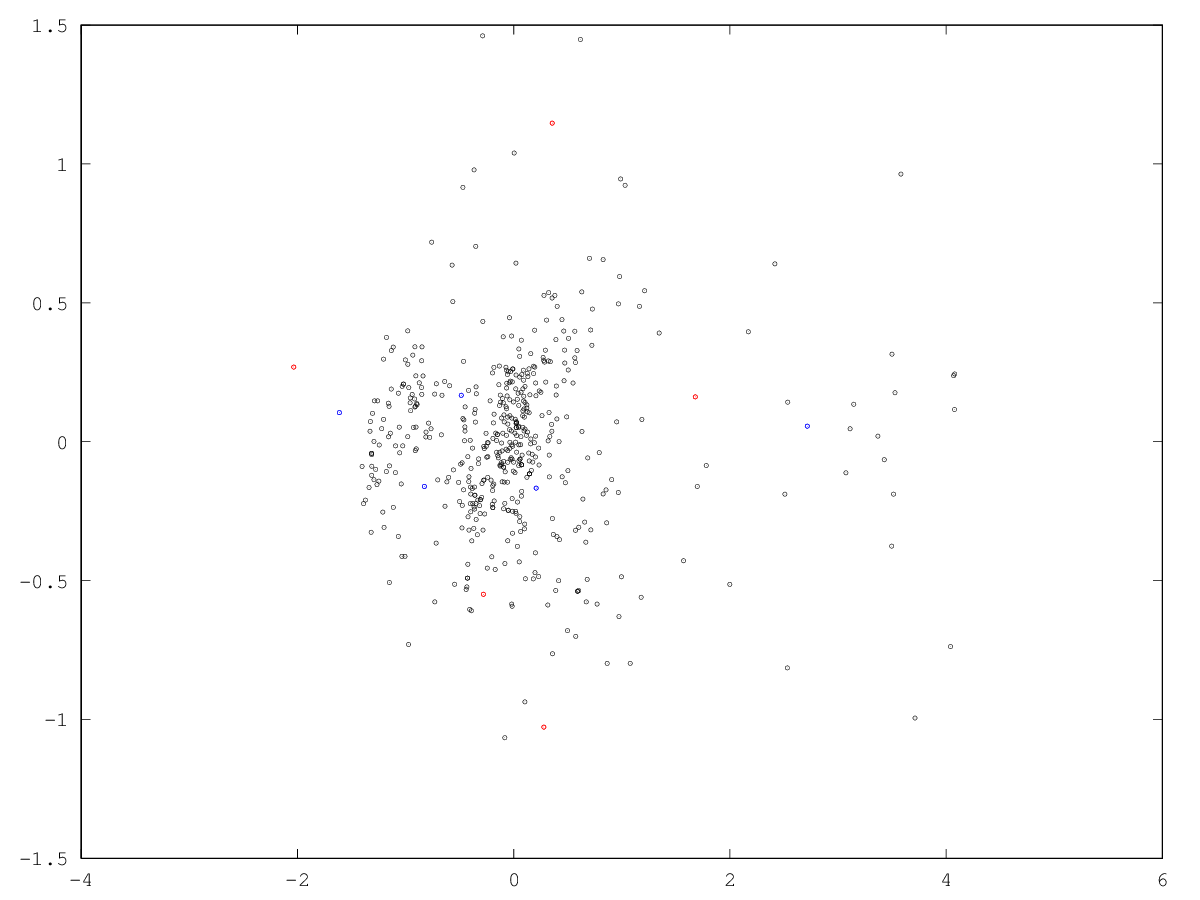
\includegraphics[width=0.85\textwidth]{kyle_base.png}
  \label{fig:kyle_base}
\end{figure}

We also plotted silhouette plots of the UCI accelerometer dataset , see Figs. ~\ref{fez_silhouette_base}, ~\ref{fez_silhouette_kmeans}, ~\ref{fez_silhouette_fuzzy}.

\begin{figure}[h!]
  \caption{Accelerometer dataset, real labels}
  \centering
    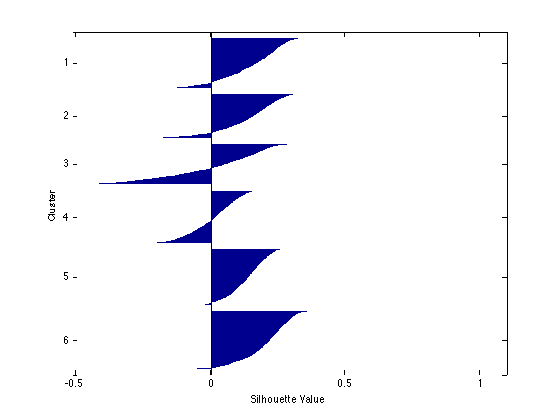
\includegraphics[width=0.85\textwidth]{fez_silhouette_real_labels.png}
  \label{fig:fez_silhouette_base}
\end{figure}

\begin{figure}[h!]
  \caption{K-means clustering silhouette}
  \centering
    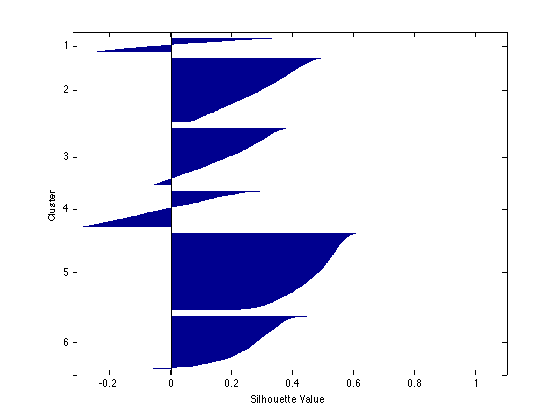
\includegraphics[width=0.85\textwidth]{fez_silhouette_kmeans.png}
  \label{fig:fez_silhouette_kmeans}
\end{figure}

\begin{figure}[h!]
  \caption{Fuzzy clustering silhouette}
  \centering
    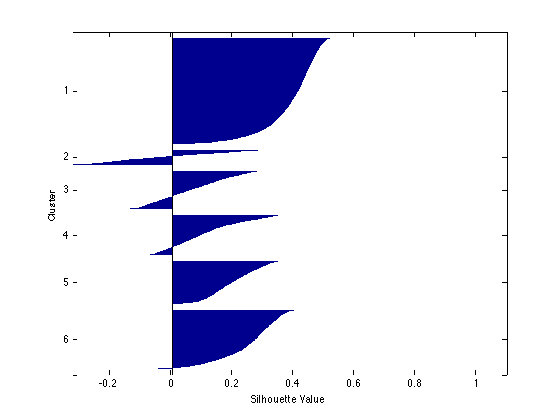
\includegraphics[width=0.85\textwidth]{fez_silhouette_fuzzy.png}
  \label{fig:fez_silhouette_fuzzy}
\end{figure}

\section*{Conclusion}
There are many issues when using a clustering algorithm, and some of our key concerns are listed below.

\begin{itemize}
\item After performing K-Means or C-Means clustering, and obtaining a cluster set $[C_1, C_2,\ldots,C_n]$, how do we know which cluster set corresponds to a label set?
\item Besides PCA, how else can we evaluate high dimensional datasets and how do we represent them?
\item What happens if our C-means or K-means algorithm can’t figure out the exact number of classes?
\item How do we improve K-means and C-Means?
\item How do we deal with peculiarities in our dataset?
\end{itemize}

We plan to tackle some of these topics in the next homework - others are outstanding research topics in the clustering field.

\section*{Appendix: 2D Cluster Code}
\begin{lstlisting}
path='/Users/Hafez/Documents/MATLAB/Kaggle Biometric Data';
cd([path,'/Homework 1 Data']);
flameData=importdata('flame.txt');
cd(path);
X=[flameData(:,1),flameData(:,2)];
realClusters=flameData(:,3);

% figure 1:  1st original dataset:
figure (1);
plot(X(realClusters==1,1),X(realClusters==1,2),'ro');
hold on
plot(X(realClusters==2,1),X(realClusters==2,2),'go');


%performing K-Means:
[kmeans_clusters,kmeans_centers]=kmeans(X,2);
figure (2);
plot(X(kmeans_clusters==1,1),X(kmeans_clusters==1,2),'ro');
hold on
plot(X(kmeans_clusters==2,1),X(kmeans_clusters==2,2),'go');
hold on
plot(kmeans_centers(1,1),kmeans_centers(1,2),'rx','lineWidth',5);
hold on
plot(kmeans_centers(2,1),kmeans_centers(2,2),'gx','lineWidth',5);
legend('cluster 1', 'cluster 2','center 1','center 2');


%performing fuzzy c-means:
[fcm_centers,fcm_memberships]=fcm(X,2);

[maxVal,fcm_clusters]=max(fcm_memberships);
figure(3);
plot(X(fcm_clusters==1,1),X(fcm_clusters==1,2),'ro');
hold on
plot(X(fcm_clusters==2,1),X(fcm_clusters==2,2),'go');
hold on
plot(fcm_centers(1,1),fcm_centers(1,2),'rx','lineWidth',5);
hold on
plot(fcm_centers(2,1),fcm_centers(2,2),'gx','lineWidth',5);
legend('cluster 1', 'cluster 2','center 1','center 2');


%performing K-Means:
[kmeans_clusters,kmeans_centers]=kmeans(X,2,'Replicates',10);
figure (4);
plot(X(kmeans_clusters==1,1),X(kmeans_clusters==1,2),'ro');
hold on
plot(X(kmeans_clusters==2,1),X(kmeans_clusters==2,2),'go');
hold on
plot(kmeans_centers(1,1),kmeans_centers(1,2),'rx','lineWidth',5);
hold on
plot(kmeans_centers(2,1),kmeans_centers(2,2),'gx','lineWidth',5);
legend('cluster 1', 'cluster 2','center 1','center 2');


%performing fuzzy c-means:
[fcm_centers,fcm_memberships]=fcm(X,2,1.2);

[maxVal,fcm_clusters]=max(fcm_memberships);
figure(5);
plot(X(fcm_clusters==1,1),X(fcm_clusters==1,2),'ro');
hold on
plot(X(fcm_clusters==2,1),X(fcm_clusters==2,2),'go');
hold on
plot(fcm_centers(1,1),fcm_centers(1,2),'rx','lineWidth',5);
hold on
plot(fcm_centers(2,1),fcm_centers(2,2),'gx','lineWidth',5);
legend('cluster 1', 'cluster 2','center 1','center 2');
\end{lstlisting}

\section*{Appendix: 7 Cluster Code}
\begin{lstlisting}
sth='/Users/Hafez/Documents/MATLAB/Kaggle Biometric Data';
cd([path,'/Homework 1 Data']);
dataSet=importdata('Aggregation.txt');
cd(path);

data_x=dataSet(:,1);
data_y=dataSet(:,2);
X=[data_x,data_y];
data_labels=dataSet(:,3);

figure(1);
plot(X(:,1),X(:,2),'o');
hold on
title('Original Dataset');
xlabel('x');
ylabel('y');

grid on;


%performing K-Means:
[kmeans_idx,kmeans_centers]=kmeans(X,7,'Replicates',10,'distance','sqEuclidean');

figure(2);
plot(X(kmeans_idx==1,1),X(kmeans_idx==1,2),'bo');
hold on
plot(kmeans_centers(1,1),kmeans_centers(1,2),'rx','lineWidth',3);
hold on
plot(X(kmeans_idx==2,1),X(kmeans_idx==2,2),'ro');
hold on
plot(kmeans_centers(2,1),kmeans_centers(2,2),'gx','lineWidth',3);
hold on
plot(X(kmeans_idx==3,1),X(kmeans_idx==3,2),'go');
hold on
plot(kmeans_centers(3,1),kmeans_centers(3,2),'kx','lineWidth',3);
hold on
plot(X(kmeans_idx==4,1),X(kmeans_idx==4,2),'ko');
hold on
plot(kmeans_centers(4,1),kmeans_centers(4,2),'cx','lineWidth',3);
hold on
plot(X(kmeans_idx==5,1),X(kmeans_idx==5,2),'co');
hold on
plot(kmeans_centers(5,1),kmeans_centers(5,2),'mx','lineWidth',3);
hold on
plot(X(kmeans_idx==6,1),X(kmeans_idx==6,2),'mo');
hold on
plot(kmeans_centers(6,1),kmeans_centers(6,2),'yx','lineWidth',3);
hold on
plot(X(kmeans_idx==7,1),X(kmeans_idx==7,2),'yo');
hold on
plot(kmeans_centers(7,1),kmeans_centers(7,2),'bx','lineWidth',3);
hold on

%performing fuzzy - cmeans:
[cmeans_centers,cmeans_members]=fcm(X,7);
[dummyVar,cmeans_idx]=max(cmeans_members,[],1);
figure(3);
plot(X(cmeans_idx==1,1),X(cmeans_idx==1,2),'bo');
hold on
plot(cmeans_centers(1,1),cmeans_centers(1,2),'rx','lineWidth',3);
hold on
plot(X(cmeans_idx==2,1),X(cmeans_idx==2,2),'ro');
hold on
plot(cmeans_centers(2,1),cmeans_centers(2,2),'gx','lineWidth',3);
hold on
plot(X(cmeans_idx==3,1),X(cmeans_idx==3,2),'go');
hold on
plot(cmeans_centers(3,1),cmeans_centers(3,2),'kx','lineWidth',3);
hold on
plot(X(cmeans_idx==4,1),X(cmeans_idx==4,2),'ko');
hold on
plot(cmeans_centers(4,1),cmeans_centers(4,2),'cx','lineWidth',3);
hold on
plot(X(cmeans_idx==5,1),X(cmeans_idx==5,2),'co');
hold on
plot(cmeans_centers(5,1),cmeans_centers(5,2),'mx','lineWidth',3);
hold on
plot(X(cmeans_idx==6,1),X(cmeans_idx==6,2),'mo');
hold on
plot(cmeans_centers(6,1),cmeans_centers(6,2),'yx','lineWidth',3);
hold on
plot(X(cmeans_idx==7,1),X(cmeans_idx==7,2),'yo');
hold on
plot(cmeans_centers(7,1),cmeans_centers(7,2),'bx','lineWidth',3);
hold on
\end{lstlisting}
\section*{Appendix: Biometrics Code}
\begin{lstlisting}
num_clusters = 5;
X = dlmread('train.csv', ',' , [1,1,500,3]);
fuzzy_centers = fcm(X, num_clusters, [25,1E-5,0]);
[unused, kmeans_centers] = kmeans(X, num_clusters)

% Data
% Normalization
mu = mean(X);
c = bsxfun(@minus, X, mu);
% Eigenvector decomposition (sorted into descending order)
covar = cov(c);
[U,S,V] = svd(covar);
reduced_X = c*V(:, 1:2);

% Kmeans clusters
% Normalization
mu = mean(kmeans_centers);
c = bsxfun(@minus, kmeans_centers, mu);
% Eigenvector decomposition (sorted into descending order)
covar = cov(c);
[U,S,V] = svd(covar);
reduced_kmeans = c*V(:, 1:2);

% Fuzzy clusters
% Normalization
mu = mean(fuzzy_centers);
c = bsxfun(@minus, fuzzy_centers, mu);
% Eigenvector decomposition (sorted into descending order)
covar = cov(c);
[U,S,V] = svd(covar);
reduced_fuzzy = c*V(:, 1:2);

%Plotting
clf
hold on
scatter(reduced_X(:,1),reduced_X(:,2),'black')
scatter(reduced_fuzzy(:,1),reduced_fuzzy(:,2),'red')
scatter(reduced_kmeans(:,1),reduced_kmeans(:,2),'blue')
%Scatter legend is bugged in my version.
%Sigh
%http://savannah.gnu.org/bugs/?33463
legend({'data', 'fuzzy','kmeans'});
legend('show')
print -dpng kyle_base.png
hold off    
\end{lstlisting}
\begin{thebibliography}{9}

\bibitem{ClusterAgg}
  A.H.M. and P. T. Gionis, 
  \emph{Clustering Aggregation}
  ACM Transactions on Knowledge Discovery form Data, 
  2007 

\bibitem{2DClust}
  University of Eastern Finland
  \emph{Clustering Datasets}
  http://cs.joensuu.fi/sipu/datasets/,
  accessed 9/19/2013

\bibitem{UCIML}
  UCI Machine Learning Repository
  \emph{Human Activity Recognition}
  http://archive.ics.uci.edu/ml/datasets/Human+Activity+Recognition+Using+Smartphones
  accessed 9/19/2013

\bibitem{Kaggle}
  Kaggle 
  \emph{Accelerometer Biometric Competition}
  https://www.kaggle.com/c/accelerometer-biometric-competition/data
  accessed 9/19/2013

\end{thebibliography}
\end{document}
